%!TEX root = IS_0_s1234567_s2345678.tex


\section{Exercise 1}
\subsection{Step 1}

We implemented an autoencoder deigned for CIFAR-10 image data. The code is structured in 4 classes: encoder.py, decoder.py, autoencoder,py and train autoencoder.py. A random seed was used to ensure reproducibility.

The Encoder module consists of 4 convolutional layers. For downsampling, we used stride-2 convolutions in the first 3 layers. For the Decoder module, we also used 4 convolutional layers and for upsampling we used transposed convolutions with a stride of 2. The final layer uses sigmoid activation function to match the input image normalization range between [0,1].

The training script (main.py) was adapted from the last assignment with some modifications related to the loss function, the visualization logic and how the model is saved. Below, you can find the autoencoder losses plots and reconstructions for L1 and L2. The visualization code allows for the model to select a specific test batch index (default is batch 3) and displays 10 original and reconstructed images. The script also saves the separate encoder weights in encoder.pth in the checkpoint autoenc folder which is generated once you start the training process (a copy of this folder will also be provided just in case).

\begin{figure}[H] 
    \centering
    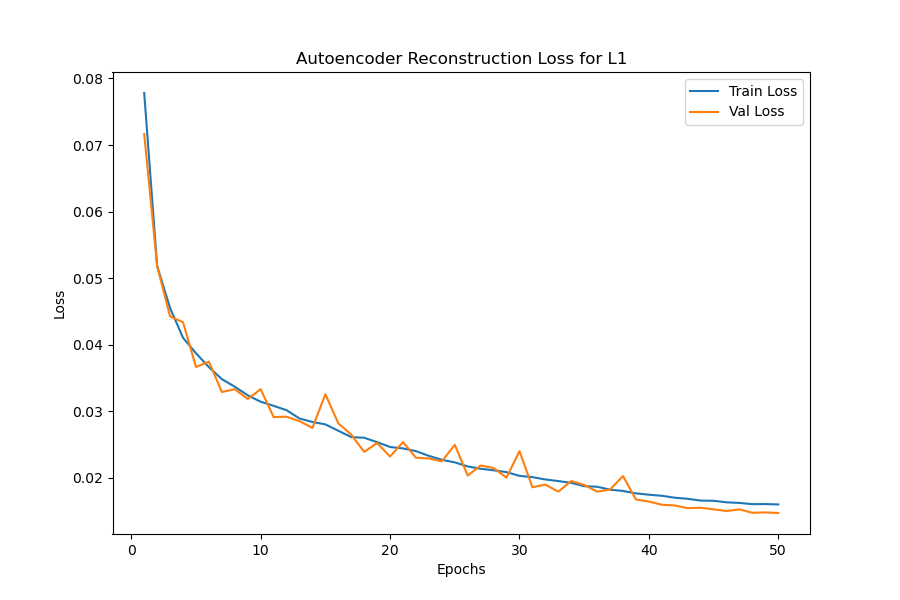
\includegraphics[width=0.8\textwidth]{assignment_2/report/images/ex1_autoencoder_loss_l1.png} 
    \caption{Autoencoder Loss for L1}
\end{figure}

\begin{figure}[H] 
    \centering
    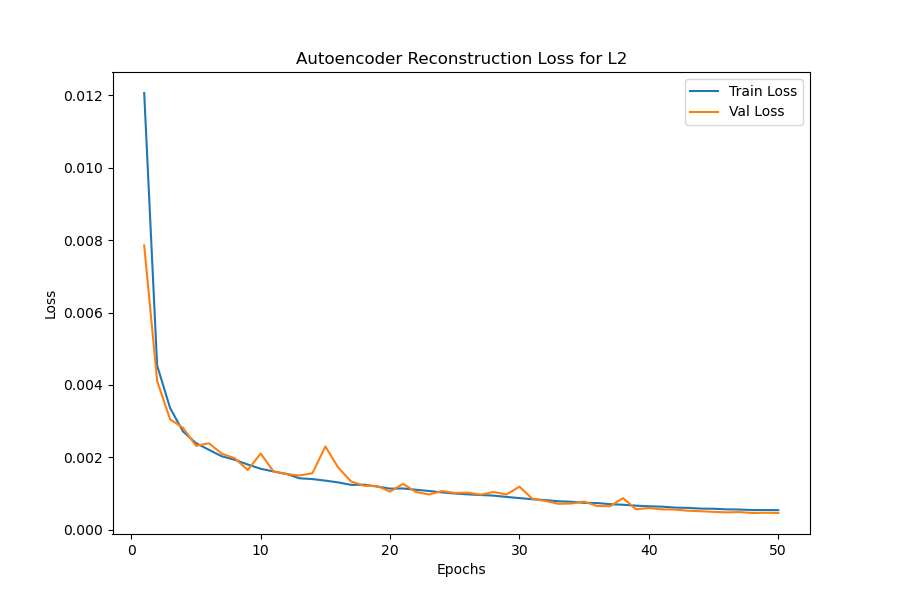
\includegraphics[width=0.8\textwidth]{assignment_2/report/images/ex1_autoencoder_loss_l2.png} 
    \caption{Autoencoder Loss for L2}
\end{figure}

From the plots above, we can see that L2 loss penalizes large errors by squaring them. This way the model is encouraged to minimize the maximum error from all pixels which gives a smoother validation performance. On the other hand, L1 loss doesn't penalize large errors as harshly which results in more fluctuations as the model encounters less-common data points. Both loss functions achieve convergence and show the model is learning successfully.

\begin{figure}[H] 
    \centering
    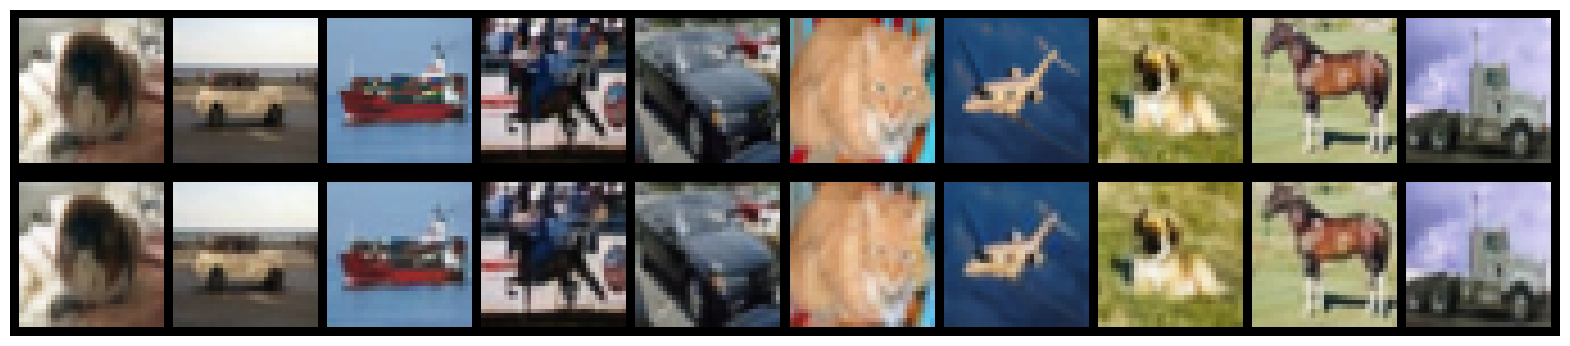
\includegraphics[width=0.95\textwidth]{assignment_2/report/images/ex1_reconstructions_l1.png} 
    \caption{Reconstructions for L1}
\end{figure}

\begin{figure}[H] 
    \centering
    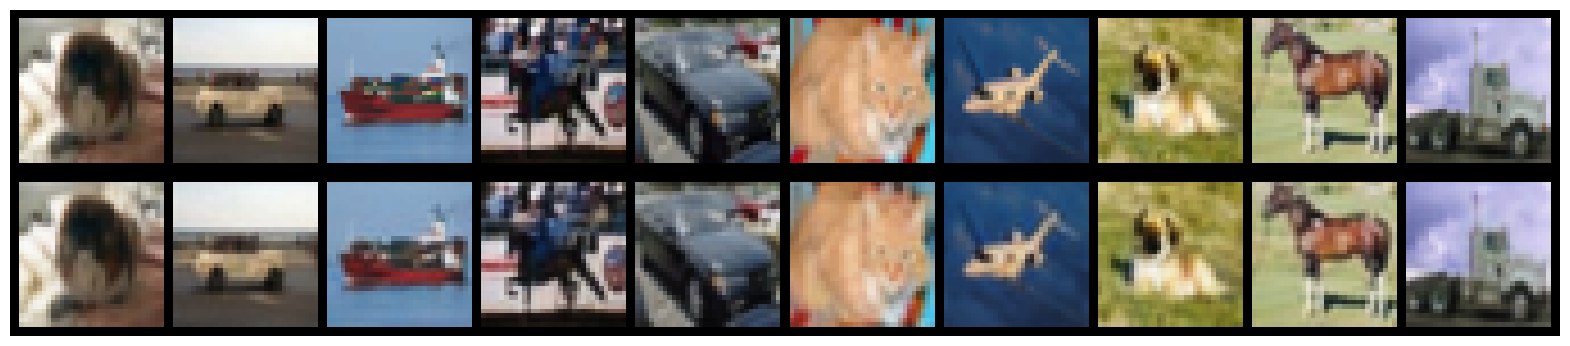
\includegraphics[width=0.95\textwidth]{assignment_2/report/images/ex1_reconstructions_l2.png} 
    \caption{Reconstructions for L2}
\end{figure}

From the image reconstructions above we can see that the bottom rows (reconstructions) are very similar to their corresponding original images on top rows. The only differences we noticed were regarding to colours, for example, the cargo on the ship is more colourful in the original image than the cargo in the reconstructions. Between L1 and L2 reconstructions, we can't see any differences with the naked eye, showing that even though L2 behaved better in the plots, the differences in the actual reconstructed images are insignificant.

\subsection{Step 2}





